\chapter{Negotiation Skills}

Following Joseph Hadzima's handoff in this MIT OpenCourseWare session, Mindy Garber treats negotiation as part of the operating structure of a new venture, not as an after-the-fact legal ritual. The present companion notes, curated by LazyingArt LLC, keep close to her order of presentation and make the lecture's implicit mathematics explicit only where that helps: we identify parties, surface interests, widen the space of options, and keep track of the relationships on which the company must continue to live.

\section{Why Negotiation Belongs in a Startup Course}

Garber opens by placing the subject inside the failure mechanics of young companies. Ventures, she says, do not merely fail because a technology does not work or because the financing is weak. Very often they fail because the founders cannot keep working together, and the result is not only interpersonal disappointment but wasted intellectual property. This is the right opening move, because it tells us why negotiation belongs here at all. It is part of venture formation itself.

Her self-description as both engineer and mediator sharpens the point. The engineer gathers facts and seeks an optimal solution; the mediator helps people have a conversation they were not yet able to have. In startup life we need both. We need disciplined analysis, but we also need a method for making the relevant human variables visible before they break the enterprise.

As editorial shorthand, and not as notation used on Garber's slides, we may compress a negotiation into the tuple
\begin{equation}
N = (\mathcal{P}, \{I_p\}_{p\in\mathcal{P}}, O, R),
\end{equation}
where \(\mathcal{P}\) is the set of parties, \(I_p\) is the interest set of party \(p\), \(O\) is the option space, and \(R\) denotes the relationship and reputation constraints that survive the present meeting.

\begin{definition}
In these notes, a negotiation is any structured attempt by a set of parties \(\mathcal{P}\) to move from partially conflicting aims toward an outcome in \(O\), under the constraint that each party carries interests \(I_p\) and that the relationship term \(R\) is usually nontrivial.
\end{definition}

The final clause matters. Garber does not begin with term sheets or courtroom tactics. She begins with the much more primitive fact that people in a venture must keep speaking, deciding, revisiting, and working together.

\subsection{Question \& Answer}

\paragraph{Question.} Why is negotiation a venture skill rather than a legal afterthought?

\paragraph{Answer.} Because the venture is already negotiating before any lawyer appears. Cofounders negotiate motives, sacrifice, ownership, roles, and future authority; teammates negotiate culture and accountability; companies negotiate with customers, collaborators, and partners. If those conversations fail, the company can fail while the technology is still intact.

\section{Win-Lose, Collaboration, and Reputation}

Garber's first conceptual split is simple and important. There are many schools of thought about negotiation, but at the lecture's level they fall into two broad modes:
\begin{equation}
\mathrm{mode}(N) \in \{\text{win-lose},\ \text{collaborative problem solving}\}.
\end{equation}

In the win-lose picture, the exchange is treated as zero-sum. If one side gets more, the other side gets less. The relationship is incidental. In the collaborative picture, the parties are working on a problem together, and the relationship is itself part of what must be preserved. Garber aligns herself explicitly with the second model, drawing on the \emph{Getting to Yes} tradition and on her own experience as a mediator.

The lecture does not present this as mere moral uplift. The point is structural. Startup life is almost never one-and-done. The same person may later be a customer, a vendor, an investor, an acquirer, a colleague at another firm, or simply a node in the reputation network through which future opportunities travel. In our notation, the relationship term is almost never absent:
\begin{equation}
R \neq \varnothing.
\end{equation}

This is why Garber insists that principled negotiation matters. Your reputation precedes you, and today's extractive victory may become tomorrow's blocked sale.

\subsection{Question \& Answer}

\paragraph{Question.} Is negotiation fundamentally adversarial or collaborative?

\paragraph{Answer.} Garber's answer is that the adversarial temptation is always present, but startup negotiations usually live inside continuing relationships, so the more faithful model is collaborative problem solving under constraint. We may have disagreements, but we usually cannot afford to behave as if the other side will disappear forever.

\section{Interests, Positions, and the Expansion of Options}

Here the lecture finds its analytic spine. Garber asks the question that drives everything which follows: what are your interests? She glosses this broadly as needs, goals, hopes, and fears. The reason is immediate. Many people cannot solve a problem because they have not yet clarified what they actually want.

\begin{definition}
A \emph{position} \(P_i\) is a stated demand, preferred term, or declared answer. An \emph{interest} \(I_i\) is the underlying need or concern that makes the position meaningful.
\end{definition}

The lecture's central logical chain can then be written as
\begin{equation}
P_i \longrightarrow I_i \longrightarrow O(I_i),
\end{equation}
where
\begin{equation}
O(I) = \{o : o \text{ satisfies the underlying interest } I\}.
\end{equation}

This is Garber's most important quasi-derivational step. Once we identify the interest beneath the position, the option space expands.

\begin{proposition}
If a stated position \(P_i\) is only one means of satisfying an underlying interest \(I_i\), then replacing \(P_i\) by \(I_i\) enlarges the visible solution set from \(\{P_i\}\) to \(O(I_i)\), with
\[
\{P_i\} \subseteq O(I_i).
\]
\end{proposition}

\begin{proof}
Garber's fence example is enough. Suppose one party says, ``I want \(\$500\).'' That is the position. If we ask why, we learn that the fence was damaged and must be repaired. The interest is not intrinsically the cash; it is the repair. Once the interest is explicit, direct repair becomes another admissible option. So the single visible candidate \(\{P_i\}\) is replaced by a larger family \(O(I_i)\).
\end{proof}

Her examples are concrete:
\begin{align}
P_{\text{fence}} &= \$500, &
I_{\text{fence}} &= \text{repair the fence},\\
o_1 &= \text{cash payment}, &
o_2 &= \text{direct repair by the other side}.
\end{align}

The same structure appears in the technical example. Engineers often enter a dispute with what looks like the right answer already in hand: ``We need C++.'' Garber's point is that even this is often a position rather than an interest.
\begin{align}
P_{\text{code}} &= \text{use C++},\\
I_{\text{code}} &= \text{minimize time to an implementable system},\\
t_{\text{new language}} &\approx 6 \text{ months},\\
t_{\text{C++}} &\approx 3 \text{ weeks}.
\end{align}

Now the issue is not language loyalty. The real issue is schedule. Once that is visible, one can reason about implementation time instead of defending an answer merely because it is familiar.

A useful derivation, very close to the lecture's cadence, is therefore:

\begin{enumerate}
\item Begin with the position \(P_i\).
\item Ask why that position matters.
\item Replace the defended answer by the underlying interest \(I_i\).
\item Search over \(O(I_i)\) rather than over the original statement.
\item Compare options by how well they satisfy the interest, not by how closely they resemble the opening demand.
\end{enumerate}

Garber later returns to this distinction during the Sandra case, when she remarks that ``I want to raise capital'' may itself still be only a position unless we ask what that capital is for.

\subsection{Question \& Answer}

\paragraph{Question.} What is the difference between a position and an interest?

\paragraph{Answer.} A position is the thing we say we want. An interest is the reason we want it. Garber's method is to keep asking why until the answer stops sounding like a bargaining move and starts sounding like a need, a fear, a constraint, or an aim. Only then do we see the real option space.

\section{Founder Negotiation: First Questions and the Circle of Interests}

Only after building the position-interest mechanism does Garber narrow to startup life. The first founder negotiation is not yet about equity or titles. It is diagnostic. She gives the class three opening questions:
\begin{equation}
Q_0 = (\text{motivation},\ \text{success},\ \text{sacrifice}).
\end{equation}

In words: Why are you doing this? What does success look like? What are you giving up?

The third question is the most revealing because it anchors motive in cost. Someone may be giving up graduate school, a job at Google, or some other valuable path. That sacrifice tells us how much risk the person thinks he or she is taking, and therefore what future tensions may later emerge around pace, control, or reward.

Garber insists on a second step: active listening. The point is not merely to ask the question and move on. The partner should restate the answer in altered words so that both sides feel heard. Before any formal agreement, the cofounders need evidence that they can hear one another accurately.

The lecture then condenses this exercise into its clearest visual method.

\begin{figure}[h]
\centering

\includegraphics[width=0.95\linewidth]{lecture_07_figure_02.png}
\caption{Circle-of-interests map for two founders.}
\end{figure}

The slide is important because the circle itself is blank. The content is outside the center, in the separate lists. One founder wants entrepreneurial success, profit, impact, and a chance to use technical skill in a startup. The other wants to solve an identified problem, learn technology, challenge personal limits, and deepen detail and execution. The point is not to average these motives. The point is to get them onto one page before conflict arrives.

\begin{figure}[h]
\centering
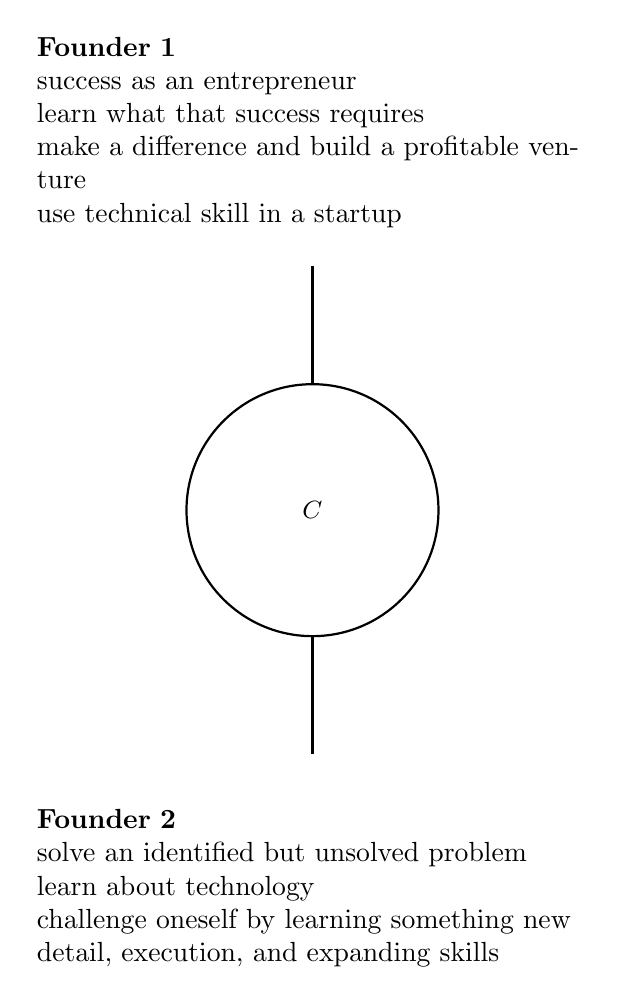
\begin{tikzpicture}[x=1cm,y=1cm]
\draw[thick] (0,0) circle (1.6);
\node at (0,0) {\small \(C\)};
\node[align=left,text width=7cm] at (0,4.8) {\textbf{Founder 1}\\
success as an entrepreneur\\
learn what that success requires\\
make a difference and build a profitable venture\\
use technical skill in a startup};
\draw[thick] (0,3.1) -- (0,1.6);
\node[align=left,text width=7cm] at (0,-4.8) {\textbf{Founder 2}\\
solve an identified but unsolved problem\\
learn about technology\\
challenge oneself by learning something new\\
detail, execution, and expanding skills};
\draw[thick] (0,-1.6) -- (0,-3.1);
\end{tikzpicture}
\caption{Editorial redraw of the circle-of-interests method. Here \(C\) denotes the shared discussion space on which the founders place their interests.}
\end{figure}

As editorial shorthand we may write
\begin{equation}
I_{\mathrm{F1}},\ I_{\mathrm{F2}} \longrightarrow C,
\end{equation}
where \(C\) is not a contract or a company yet. It is the common page, or common conversational field, on which the parties make their motives legible.

\begin{definition}
A \emph{circle of interests} is a compact map that places the parties' distinct interest sets around a shared discussion space so that hidden motives become discussable before they harden into conflict.
\end{definition}

Garber's emphasis here is practical. In her example, the two founders had a good idea and both wanted to pursue it, but they had not actually discussed why each wanted to do so. The diagram therefore does not decorate the conversation. It stabilizes it.

\subsection{Question \& Answer}

\paragraph{Question.} How do we make hidden founder motives visible before conflict arrives?

\paragraph{Answer.} By asking the first questions, restating what we heard, and writing the answers down in a shared map. Garber's circle does not solve the disagreement automatically; it does something more basic. It prevents us from negotiating blind.

\section{From Founder Fit to Formal Agreements}

Once the founders' motives are visible, the lecture thickens. Garber turns to honest assessment, founders agreements, team agreements, culture, roles, accountability, and decision rules. The rhythm is cumulative. Each new topic is another place where hidden interests will surface sooner or later, so the smart move is to surface them early.

The honest-assessment discussion is easy to misread if we move too fast. Garber is not saying that founders must have complementary technical backgrounds from the start. Two mechanical engineers may perfectly well found a company together. Her point is that they must know what skills they do and do not bring, because the missing skills will have to enter the venture somehow.

The founders agreement then formalizes ownership, contribution, equity, and departure contingencies. Garber is especially emphatic about the problem of a founder leaving. A company cannot safely postpone the question of what happens if one person departs for graduate school or some other opportunity.

The team agreement moves from ownership to operation. Garber treats it as the internal constitution of day-to-day collaboration. It covers, among other things,

\begin{itemize}
\item culture and expected behavior,
\item meeting structure,
\item communication tools and channels,
\item roles and accountability,
\item decision procedures,
\item the language by which the team can later revisit what it previously agreed.
\end{itemize}

This last point is subtle and important. A written agreement does not only fix a rule. It creates a neutral vocabulary for later repair. Instead of accusing one another in purely personal terms, the team can say: this is what we said we would do; is it still working; if not, how shall we revise it?

The lecture then turns to the structural deadlock of equal founders:
\begin{equation}
s_1 = s_2 = 0.5.
\end{equation}

Garber does not reject the arrangement. On the contrary, she remarks that nearly everyone she sees is in a \(50\!:\!50\) structure. The problem is not that equality is impossible. The problem is that equality requires tools.

A useful editorial distinction, explicitly motivated by the classroom exchange, is
\begin{equation}
D \in \{D_{\text{one-way}},\ D_{\text{two-way}}\}.
\end{equation}
A one-way decision is hard to reverse and therefore requires slower, more explicit resolution. A two-way decision can be tested and revisited, so the team may sometimes decide, observe, and adjust.

Garber's lawyer anecdote offers a crude anti-deadlock answer:
\begin{equation}
(s_1,s_2) = (0.51, 0.49).
\end{equation}

\begin{remark}
The lecture does not treat the \(0.51/0.49\) split as a theorem of venture design. It appears as a litigation-minded lawyer's response to deadlock. Garber's own pedagogical aim is different: give founders the tools to avoid ending up in court at all.
\end{remark}

\subsection{Question \& Answer}

\paragraph{Question.} What should equal cofounders do when they disagree?

\paragraph{Answer.} Garber's answer is layered rather than magical. First, they should have a real conversation. Second, they may use neutral advice, mediation, or an agreed outside consultant. Third, they should distinguish reversible from irreversible decisions:
\begin{equation}
D_{\text{two-way}} \Rightarrow \text{test, observe, revisit}, \qquad
D_{\text{one-way}} \Rightarrow \text{slow down, deliberate, and if needed seek help}.
\end{equation}
The right tool depends on the structure of the decision, not merely on the temperature of the argument.

\section{The Sandra Case: A Negotiation Failure in Slow Motion}

Garber now slows the lecture and introduces a true MIT case. This is the chapter's major worked example because it lets us watch the method under strain.

\begin{figure}[h]
\centering

\includegraphics[width=0.95\linewidth]{lecture_07_figure_03.png}
\caption{Overview of the Sandra-undergraduates negotiation case.}
\end{figure}

The slide's order matters, so we keep it. Sandra has a prototype, but the prototype can process only one cup of crude oil at a time. Several undergraduates hear about the invention, meet Sandra, and somehow move toward the \(100\text{K}\) competition and perhaps a startup. The relationship between inventor and students is never documented. The students then invest heavily in the business plan and in industry connections. Just before the competition, Sandra considers pulling out because the invention is not yet ready.

In compact form, the case state is
\begin{align}
q_{\text{prototype}} &= 1 \text{ cup at a time},\\
A_{\text{written}} &= \varnothing,\\
\text{student investment} &= \text{already substantial},\\
\text{withdrawal point} &= \text{immediately before the competition}.
\end{align}

The class first identifies interests. The students may want experience, career opportunities, resume value, access to executives, the excitement of forming a company, and perhaps the chance to build a meaningful career around a useful technology. Sandra, by contrast, wants to protect her intellectual property, preserve control, protect her reputation in the field, and avoid declaring the invention ready when the scaling problem remains unresolved.

Garber is careful here: inferred interests are not guaranteed to be correct. Even in mediation, if she guesses an interest, the party may respond, ``No, that is not it.'' But the effort to articulate possible interests is still necessary, because without it we do not know what to offer.

The class then generates possible agreements. Several types recur:

\begin{itemize}
\item a joint venture in which Sandra licenses the invention and remains an advisor rather than a day-to-day founder,
\item an equity arrangement based on the functions required for the company rather than on one undifferentiated claim of value,
\item an IP-protective structure, perhaps involving patents or licensing,
\item a research-first path in which the parties postpone the startup and work first on scaling, grants, and technical validation.
\end{itemize}

These are not random ideas. They are precisely what the \(P_i \to I_i \to O\) method predicts. Once the interests are named, many candidate structures appear.

The reveal is the whole point. In reality, there was no agreement. More sharply, there was never a real conversation about what the students wanted and what Sandra wanted. Garber had even offered to serve as a neutral party to help them have that conversation, but the students assumed it would somehow work out if they kept working hard enough. It did not. Sandra later took the invention and formed a company with other people.

\subsection{Question \& Answer}

\paragraph{Question.} Why did effort, enthusiasm, and opportunity still fail to produce an agreement?

\paragraph{Answer.} Because none of those things substitutes for negotiation. The students invested labor and optimism; Sandra had the invention and the control. But the parties never stabilized their interests, never documented their relationship, and never tested whether their preferred future was even the same future. In Garber's framework, the option set could not be searched because the interests were never jointly clarified.

\section{Negotiation Within and Beyond the Company}

The Sandra case leads naturally to the next scale. Once the company exists, negotiation does not disappear; it becomes more complicated.

\begin{figure}[h]
\centering

\includegraphics[width=0.95\linewidth]{lecture_07_figure_04.png}
\caption{Internal-company negotiation complications.}
\end{figure}

Garber's internal-company checklist is concise and exact. There may be more than two parties; there may be differences in ``power levels''; there may be legal ramifications; and there may be a further layer of confidentiality. In symbols, the simplest extension is
\begin{equation}
n > 2,
\end{equation}
and, with slightly richer editorial notation,
\begin{equation}
N_{\text{internal}} = (\mathcal{P}, \{I_p\}_{p\in \mathcal{P}}, O, R, L, K),
\end{equation}
where \(L\) records legal implications and \(K\) records confidentiality constraints.

Even here, Garber says, she still draws her little circle of interests.

\paragraph{The Judy case.} The internal example concerns Judy's attempt to become a marketing manager. Garber's method is to enumerate stakeholders:
\begin{equation}
S_{\text{Judy}} = \{\text{Judy},\ \text{manager},\ \text{company},\ \text{teammates}\}.
\end{equation}

Judy wants challenge, recognition, supervisory experience, and a chance to use newly acquired skills. Her manager wants employee growth but also needs the work done. The company wants revenue, leadership, employee development, and other organizational gains. Teammates may have their own promotion ambitions. The important point is that Judy's request must be framed in terms legible to all of these interests.

Garber then gives Judy a list of marketing tasks. Judy, on her own, turns the list into a spreadsheet and assigns a priority score:
\begin{equation}
w_j \in \{1,2,3\}, \qquad \text{with larger } w_j \text{ indicating greater importance.}
\end{equation}
She builds a plan and presents the work almost as if she has already begun performing the role. The negotiation succeeds because the request is not merely ``promote me.'' It is ``here is how my advancement serves the interests you already have.''

\paragraph{The Little Inc/Big Inc case.} The external-company example is more elaborate but uses the same machinery. Little Inc has a vague fixed-cost contract with Big Inc. Big Inc later cancels the contract for its own financial reasons and asks for money back. Little Inc does not rush into the meeting with arguments. Instead it first enumerates stakeholders:
\begin{equation}
S_{\text{contract}} =
\{\text{sales executive},\ \text{service manager},\ \text{CFO},\ \text{Big Inc contacts}\}.
\end{equation}

The sales executive worries about commission and follow-on business. The service side worries about reputation and the customer relationship. The CFO worries about cash flow, revenue recognition, fairness, and not being overwhelmed by a much larger company. Big Inc likely worries about its own reputation, possible legal exposure, internal blame, and the judgment of the people who signed the contract.

Garber's team then constructs what she calls a solution space, or zone of solution:
\begin{equation}
Z = \{a : a \text{ is acceptable under the parties' interests and constraints}\}.
\end{equation}

The lecture's operative derivation is straightforward:

\begin{enumerate}
\item List the stakeholders on our side and the other side.
\item Identify substantive interests, reputational interests, legal concerns, and escalation thresholds.
\item Ask what outcomes remain fair, survivable, and relationship-preserving.
\item Build \(Z\) before the meeting begins.
\item Compare the first offer to \(Z\), not to the ego's desire to keep bargaining.
\end{enumerate}

This leads to one of Garber's most practically surprising claims. Big Inc makes an opening demand. Little Inc's CFO immediately says yes. The room is startled: what kind of negotiation is that? Garber's answer is that the team had already done the real work. The first offer was better than expected, was inside the acceptable region, preserved the relationship, and avoided escalation. In that setting,
\begin{equation}
a_{\text{first}} \in Z \Longrightarrow \text{accepting may be wiser than bargaining for sport.}
\end{equation}

Garber reinforces the point with the 3M maxim that sometimes the first offer is the best offer. This is not passivity. It is disciplined precomputation.

\subsection{Question \& Answer}

\paragraph{Question.} Should we explicitly share our interests with the other side?

\paragraph{Answer.} Garber's answer is qualified. Interests can be used as weapons if we reveal them naively. But the lecture's closing stories argue that selective disclosure can change the negotiation entirely. In the acquisition-style meeting, the buyer leads with the other side's possible interests, and the conversation opens. In the IBM--3M story, once one side finally states its interests, the other side reciprocates and movement begins. Editorially we may write
\begin{equation}
I_{\text{shared}} \subseteq I_{\text{all}},
\end{equation}
where \(I_{\text{shared}}\) consists of the interests that help define the joint problem. Garber's practical rule is: do not disclose vulnerabilities merely because they are true, but do disclose the interests that make constructive agreement easier to find.

The final exchange in the lecture sharpens the same point further. If unexpected people appear in the room, their interests may differ from the institution's generic interests. The right move is often simply to ask: what is important to you, what are you trying to accomplish, what would be helpful? If they will not answer, then the negotiation space itself becomes harder to map. But if they do answer, we may discover something of low value to us and high value to them, which is precisely the kind of asymmetry from which workable agreements are built.

\section{Summary}

Garber closes not with a new theorem but with a disciplined summary. Understand the interests of your cofounder. Document decisions and revisit them, because companies change quickly. Prepare before negotiations by mapping parties, interests, and acceptable outcomes. Then listen during the meeting, because new interests may emerge that alter the option space.

Those closing instructions are entirely consistent with the chapter's analytic form. We began with the claim that startup failure is often a failure of relationships. We then saw that the practical mathematics of negotiation is light but real:
\[
\text{parties} \longrightarrow \text{interests} \longrightarrow \text{options} \longrightarrow \text{agreement under relationship constraints}.
\]
Hadzima's closing anecdote reinforces the same lesson from the other side of the table: even the people across from us may need time to discover their own internal interests before a serious negotiation can begin.